\documentclass[11pt,a4paper,oneside]{report}
\usepackage[left=23mm,right=21mm,top=22mm,bottom=23mm,headheight=15pt]{geometry}
\usepackage{fontspec}
\setmainfont{DejaVu Serif}
\setsansfont{DejaVu Sans}
\setmonofont[Scale=0.80]{DejaVu Sans Mono}
\usepackage{unicode-math}
\setmathfont{Latin Modern Math}
\usepackage{amsmath}
\usepackage{xcolor}
\definecolor{ink}{HTML}{243C46}
\definecolor{teal}{HTML}{167D8D}
\definecolor{blue}{HTML}{3464A0}
\definecolor{amber}{HTML}{A97A22}
\usepackage{graphicx}
\setkeys{Gin}{keepaspectratio}
\usepackage{float,caption}
\floatplacement{figure}{H}
\captionsetup{font=small,labelfont={bf,sf},labelsep=period,skip=7pt}
\renewcommand{\figurename}{Hình}
\renewcommand{\tablename}{Bảng}
\usepackage{longtable,booktabs,array,calc}
\usepackage{etoolbox}
\AtBeginEnvironment{longtable}{\small\renewcommand{\arraystretch}{1.15}}
\usepackage[most]{tcolorbox}
\newtcolorbox{learningbox}[3][]{enhanced,breakable,colback=#2!5!white,colframe=#2!60!white,
  coltitle=ink,colbacktitle=#2!11!white,fonttitle=\sffamily\bfseries\small,
  title={#3},boxrule=0.45pt,arc=1.5mm,left=3mm,right=3mm,top=2mm,bottom=2mm,
  before skip=9pt,after skip=9pt,#1}
\usepackage{setspace}
\setstretch{1.12}
\setlength{\parindent}{0pt}
\setlength{\parskip}{4pt}
\setlength{\emergencystretch}{3em}
\widowpenalty=10000
\clubpenalty=10000
\raggedbottom
\usepackage{titlesec}
\titleformat{\chapter}[display]{\sffamily\bfseries\color{ink}}
  {\fontsize{11}{13}\selectfont\color{teal}CHẶNG \thechapter}{9pt}{\fontsize{23}{28}\selectfont}
\titlespacing*{\chapter}{0pt}{0pt}{16pt}
\titleformat{\section}{\sffamily\bfseries\large\color{teal}}{\thesection}{0.6em}{}
\titlespacing*{\section}{0pt}{13pt}{6pt}
\titleformat{\subsection}{\sffamily\bfseries\color{ink}}{\thesubsection}{0.6em}{}
\usepackage{enumitem}
\setlist{topsep=4pt,itemsep=3pt,parsep=0pt,leftmargin=1.5em}
\providecommand{\tightlist}{\setlength{\itemsep}{2pt}\setlength{\parskip}{0pt}}
\usepackage{fvextra}
\DefineVerbatimEnvironment{verbatim}{Verbatim}{breaklines,breakanywhere,fontsize=\small}
\usepackage{xurl}
\usepackage[unicode,colorlinks=true,linkcolor=teal,urlcolor=blue,bookmarksopen=false]{hyperref}
\hypersetup{pdftitle={Học tuần tự đề tài Degron Footprint},
  pdfauthor={Nguyễn Thanh Trọng},pdfsubject={Bằng chứng và hướng nghiên cứu tới 03/11/2026},
  pdfkeywords={degron,Delta PSI,learning,full-PSI,protein}}
\usepackage{bookmark}
\usepackage{fancyhdr}
\pagestyle{fancy}
\fancyhf{}
\fancyhead[L]{\sffamily\footnotesize\color{teal}DEGRON FOOTPRINT · TÀI LIỆU HỌC}
\fancyhead[R]{\sffamily\footnotesize\color{ink}03/11/2026}
\fancyfoot[C]{\sffamily\small\thepage}
\renewcommand{\headrulewidth}{0.3pt}
\fancypagestyle{plain}{\fancyhf{}\fancyfoot[C]{\sffamily\small\thepage}\renewcommand{\headrulewidth}{0pt}}
\renewcommand{\contentsname}{Lộ trình và mục lục}
\renewcommand{\listfigurename}{Danh mục hình}
\setcounter{tocdepth}{1}
\setcounter{secnumdepth}{1}
\makeatletter
\renewcommand*\l@section{\@dottedtocline{1}{1.5em}{3.1em}}
\renewcommand*\l@figure{\@dottedtocline{1}{1.5em}{3.1em}}
\makeatother
\usepackage{tikz}
\begin{document}
\begin{titlepage}
\color{ink}\sffamily
{\small CT553H · KỸ THUẬT PHẦN MỀM · ĐẠI HỌC CẦN THƠ}\par
\vspace{12mm}
{\color{teal}\rule{\textwidth}{1.3pt}}\par
\vspace{9mm}
{\fontsize{13}{17}\selectfont TÀI LIỆU HỌC TUẦN TỰ}\par
\vspace{7mm}
{\fontsize{34}{40}\selectfont\bfseries DEGRON\\FOOTPRINT}\par
\vspace{9mm}
{\fontsize{17}{23}\selectfont Từ phép đo sinh học\\đến mô hình và công cụ nghiên cứu}\par
\vspace{13mm}
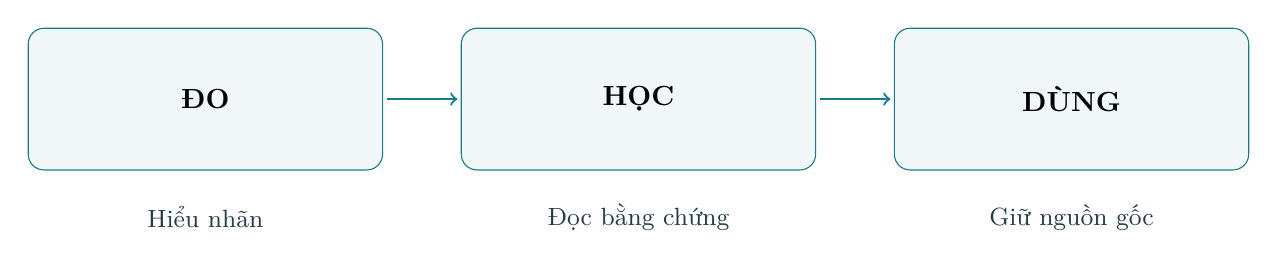
\begin{tikzpicture}[x=1mm,y=1mm]
  \foreach \x/\name/\sub in {0/ĐO/Hiểu nhãn,55/HỌC/Đọc bằng chứng,110/DÙNG/Giữ nguồn gốc}{
    \node[draw=teal,fill=teal!6,rounded corners=2mm,minimum width=45mm,minimum height=18mm] at (\x+22,0) {\bfseries\name};
    \node[font=\small,text=ink] at (\x+22,-15) {\sub};
  }
  \draw[->,thick,teal] (45,0)--(54,0);
  \draw[->,thick,teal] (100,0)--(109,0);
\end{tikzpicture}
\vfill
\begin{learningbox}{teal}{Phạm vi của bản học}
Khái niệm được giải thích trước khi dùng; kết quả gắn đối chứng và giới hạn.
Train local đang dở chỉ trình bày hướng đi và lý do lựa chọn.
\end{learningbox}
\vspace{4mm}
{\normalsize Nguyễn Thanh Trọng · GVHD: TS. Hồ Quang Thái}\par
\vspace{3mm}
{\small Mốc bằng chứng: 03/11/2026 · Tài liệu học riêng của đề tài}\par
\end{titlepage}
\pagenumbering{roman}
\tableofcontents
\clearpage
\listoffigures
\clearpage
\pagenumbering{arabic}
$body$
\end{document}
